\documentclass[11pt]{article}
\usepackage[T1]{fontenc}
\usepackage[margin=.74in]{geometry}
\usepackage{amsmath,amssymb,amsthm,booktabs,tikz}
\usepackage[hidelinks]{hyperref}
\newtheorem{theorem}{Theorem}
\newcommand{\Q}{\mathbb Q}
\newcommand{\F}{\mathbb F}
\newcommand{\Gal}{\operatorname{Gal}}
\newcommand{\Fr}{\operatorname{Frob}}
\title{The cubic field of discriminant \(-3\cdot269^2\) in the 3-torsion of elliptic curve 269a1}
\author{AI-produced mathematics (GPT-6.2 Astra)}
\date{22 November 2026}
\begin{document}
\maketitle
\begin{abstract}
Fukuda and Yoshikawa identify the three pairings of the four lines of elliptic
3-torsion with the cube roots of the discriminant. For Cremona's curve 269a1
this realizes the splitting field of \(X^3-269\) as the quotient of its
3-division field by a quaternion group of order eight. We give rational
polynomials for the quartic line field and the sextic pair field, and express
the cubic Artin function as the quotient of their Dedekind zeta functions.
A quadratic Hecke character of conductor norm nine gives the complementary
factor. At a split prime modulo three, the cubic trace can also be read from
the dimension of the 3-torsion over the quadratic extension of its residue
field. The finite checks reproduce all 48 matrices and 166 good primes up
to 1000. No human review is recorded.
\end{abstract}

Put \(\alpha=\sqrt[3]{269}>0\), \(F=\Q(\alpha)\), \(K=\Q(\zeta_3)\) and
\(L=FK\). Let \(t(p)\) denote the trace of the two-dimensional standard
representation of \(\Gal(L/\Q)=S_3\) at \(p\nmid3\cdot269\).
It is the number of roots of \(X^3-269\) modulo \(p\), less one. In particular
it is zero for \(p\equiv2\bmod3\). At \(p\equiv1\bmod3\) it is \(2\) if 269
is a cube modulo \(p\), and \(-1\) otherwise.

\section{The elliptic realization}
Cremona's table for conductor 269 gives the curve
\[
 C:\quad y^2+y=x^3-2x-1.
\]
Its standard invariants are \(b_2=0,b_4=-4,b_6=-3,b_8=-4\), giving
\(\Delta=269\). Write \(M=\Q(C[3])\). The four lines in \(C[3]\) correspond
to the four distinct \(x\)-coordinates of nonzero 3-torsion points, the roots
of \(\psi_3(X)=3X^4-12X^2-9X-4\). Write \(h=\psi_3/3\).
The natural correspondence between pairings of these lines and cube roots of
the discriminant is due to the general theory
\cite[\S\S3.1,4.1]{FY}; the quaternion fixed field is explicit in
\cite[Lemmas 6.3.2--3]{Bisatt}.

\begin{theorem}\label{group}
The mod-three representation of \(C\) is surjective. The actions on its
four lines and on their three pairings realize
\[
 \mathrm{GL}_2(\F_3)\longrightarrow S_4\longrightarrow S_3
       =\Gal(L/\Q),\qquad M^{Q_8}=L .
\]
If \(A=\Q(x_1)\) for a root of \(h\), the field of an unordered pair of the
four lines is isomorphic over \(\Q\) to
\[
 B=F\left(\sqrt{(8-\alpha)/3}\right).
\]
\end{theorem}

\begin{proof}
For \(h=X^4+aX^2+bX+c\) the three numbers
\(z=x_ix_j+x_kx_l\), one per partition into two pairs, have polynomial
\(z^3-az^2-4cz+4ac-b^2\). Here \(a=-4,b=-3,c=-4/3\), so it is
\[
 z^3+4z^2+\tfrac{16}3z+\tfrac{37}3=(z+4/3)^3+269/27.
\]
Its splitting field is \(L\), since \(269\) is prime, the real cube root
has degree three, and the quadratic cyclotomic field supplies the other roots.
Modulo five the monic quartic becomes \(X^4+X^2+2X+2\). The remainder
of \(X^{25}-X\) modulo it is \(-X(X+1)^2\); its values at \(0,-1\) are
nonzero for the quartic. Hence it has no factor of degree one or two and is
irreducible. The projective image is transitive of degree four and surjects
onto \(S_3\). Its order divides 24 and is divisible by 12. The only index-two
subgroup of \(S_4\) is \(A_4\), whose image on the pairings has order three.
The projective image is therefore \(S_4\).

Lift a nonidentity double transposition to the mod-three image. Its determinant
is one: \(\mathrm{PSL}_2(\F_3)=A_4\) under the action on the four lines.
Its square is scalar. An element of determinant one with square \(I\) in
characteristic three is diagonalizable with both eigenvalues equal, hence
scalar. Thus the lift squares to \(-I\), proving that the central kernel
is also in the image. The preimage of the Klein four group has order eight,
with its six noncentral elements of order four and unique involution \(-I\).
It is \(Q_8\).

An unordered pair determines its sum \(u=x_i+x_j\), while its complement has
sum \(-u\). The identity \(a=z-u^2\) gives \(u^2=z+4\).
Thus the six sums have equation
\[
  3u^6-24u^4+64u^2-27=0 .
\]
The three squares are distinct and nonzero, so the six labels are distinct.
Transitivity of \(S_4\) on pairs yields degree six. Taking the real square with
\(z+4/3=-\alpha/3\) identifies the pair field as asserted.
\end{proof}

\begin{figure}[ht]
\centering
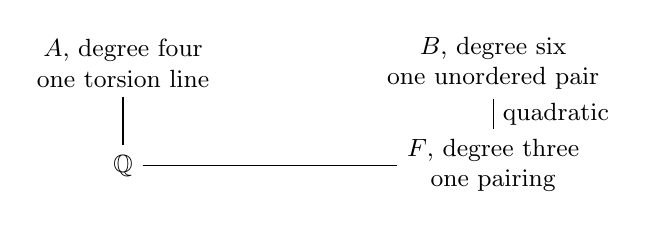
\begin{tikzpicture}[every node/.style={font=\small,align=center},x=1cm,y=1cm]
\node (A) at (0,1.2) {\(A\), degree four\\one torsion line};
\node (B) at (4.7,1.2) {\(B\), degree six\\one unordered pair};
\node (F) at (4.7,-.1) {\(F\), degree three\\one pairing};
\node (Q) at (0,-.1) {\(\Q\)};
\draw (A)--(Q);
\draw (B)-- node[right]{quadratic} (F);
\draw (Q)--(F);
\end{tikzpicture}
\caption{A pair of lines determines its complementary pair, hence a pairing.
The quartic and sextic fields correspond to distinct stabilizers. Their
zeta quotient below uses a character identity; neither field contains the other.}
\end{figure}

\section{Two explicit Hecke characters}
\begin{theorem}\label{zeta}
Let \(\theta\) be a nontrivial character of \(L/K\) and \(\eta\) the quadratic
character of \(B/F\), viewed as Hecke characters. Including the ramified Euler
factors, one has
\[
 L_K(s,\theta)=\frac{\zeta_F(s)}{\zeta_\Q(s)}
              =\frac{\zeta_B(s)}{\zeta_A(s)},\quad
 L_F(s,\eta)=\frac{\zeta_A(s)}{\zeta_\Q(s)},\quad
 \zeta_B(s)=\zeta_\Q(s)L_K(s,\theta)L_F(s,\eta).
\]
The conductor of \(\eta\) is the product of the two primes of \(F\) above 3,
of norm 9, with trivial infinite component.
\end{theorem}
\begin{proof}
Let \(P_4,P_6,P_3\) be the permutation representations on vertices, unordered
pairs and pairings. For the cycle types \(1,2,2^2,3,4\) respectively, the
characters of \(P_4\) are \(4,2,0,1,0\), those of \(P_6\) are \(6,2,2,0,0\),
and those of \(P_3\) are \(3,1,3,0,1\). Thus
\[
 P_6-P_4=P_3-1=\operatorname{Ind}_{\Gal(L/K)}^{S_3}\theta
\]
after inflation to the common Galois group. Artin formalism uses the
Frobenius operators on inertia invariants, and therefore gives the first
identity at all finite primes. The quadratic factorization
\(\zeta_B=\zeta_F L_F(\cdot,\eta)\) gives the other two.

Let \(w=(8-\alpha)/3\). Its norm is \(9\), and \(w\) is integral away
from 3. At every odd prime away from 3, \(w\) is a unit and its quadratic
extension is unramified. At 2, good reduction of \(C\) and the
prime-to-2 torsion criterion give that the full 3-division field is
unramified, hence its subfields are as well. At the real place \(8>\alpha\),
so the infinite component is trivial.

Locally \(269\equiv-1\bmod9\) is a cube in \(\Q_3\), as follows by the
logarithm on \(1+3\mathbb Z_3\). Write \(c^3=269\) in \(\Q_3\). Then
\(F\otimes\Q_3=\Q_3\times\Q_3(\zeta_3)\).
At the first factor \(8\equiv c\bmod3\), and
\(v_3(8^3-c^3)=v_3(8-c)+1=5\).
Thus the normalized valuation of \(w\) is \(3\).
At the second factor the root is \(c\zeta_3\). In
\(8-c\zeta_3=(8-c)+c(1-\zeta_3)\), the valuations are \(8\) and \(1\)
when the uniformizer has value one. Subtracting the valuation two of 3
gives \(v(w)=-1\). Both valuations are odd and the quadratic ramification is
tame, giving conductor exponent one at each prime.
\end{proof}
Both nontrivial Hecke functions are entire. Thus RH for \(\zeta_B\)
is equivalent to RH for the three displayed factors, separately.
The two Hecke functions have degrees two and three over \(\Q\).
For a discriminant check, \(|D_F|=3\cdot269^2\) by the pure cubic
discriminant formula. The relative discriminant gives
\(|D_B|=9|D_F|^2\). Conductor induction for \(L_F(s,\eta)\)
gives \(|D_A|=9|D_F|\). These yield respectively
\(217083,\ 424125260001,\ 1953747\) in absolute value.
In particular the cubic Artin function is a quotient of Dedekind functions
whose fields have degrees six and four. The elliptic curve's weight-two
\(L\)-function is a different analytic object.

\section{Reading the cubic trace over a finite field}
\begin{theorem}\label{trace}
Let \(p\nmid3\cdot269\), and \(d_j=\deg\gcd(\psi_3,X^{p^j}-X)\) over
\(\F_p\). Then
\[
 t(p)=\frac{d_1^2-4d_1+d_2}{2}.
\]
If \(p\equiv1\bmod3\) and \(e=\dim_{\F_3} C(\F_{p^2})[3]\), one also has
\[
 t(p)=3(e-1)^2-1=\frac{\#C(\F_{p^4})[3]-5}{2}.
\]
\end{theorem}
\begin{proof}
The quartic is separable at these primes. A stable pair consists of two
fixed vertices or one two-cycle. Its character is therefore
\(\binom{d_1}{2}+(d_2-d_1)/2\). Subtract the four-line character \(d_1\).
For the second statement Frobenius \(g\) lies in \(\mathrm{SL}_2(\F_3)\)
by the Weil pairing. If its image in \(S_3\) is trivial, \(g\in Q_8\):
the two scalars have \(g^2=I\) and the other six elements have \(g^2=-I\).
Then \(e=2\) or \(0\), while \(g^4=I\).
Otherwise its image is a three-cycle and \(g\) is a scalar sign times a
nonidentity unipotent matrix. Both \(g^2-I\) and \(g^4-I\) have rank one.
This gives \(e=1\) and exactly three fixed 3-torsion points over \(\F_{p^4}\).
\end{proof}
\begin{center}
\begin{tabular}{rrrrrr}
\toprule
\(p\)&\(d_1\)&\(d_2\)&\(\#C(\F_{p^2})[3]\)&\(\#C(\F_{p^4})[3]\)&\(t(p)\)\\
\midrule
7&1&1&3&3&\(-1\)\\
37&4&4&9&9&2\\
43&0&4&1&9&2\\
\bottomrule
\end{tabular}
\end{center}
The table exhibits all three quadratic torsion outcomes. The bracket \([3]\)
means the kernel of multiplication by three; divisibility of the total
number of points by nine would test a different condition.
The equality of coefficients and the all-prime zeta identities do not
supply a cancellation estimate for their sums over varying primes.

\begin{thebibliography}{9}
\bibitem{Cremona} J. E. Cremona, \emph{Algorithms for Modular Elliptic Curves},
Table 1, conductor 269, curve A1, \href{https://johncremona.github.io/ecdata/}{author's data}.
\bibitem{FY} K. Fukuda and S. Yoshikawa, \emph{The 12-th roots of the discriminant
of an elliptic curve and the torsion points}, \href{https://arxiv.org/abs/1503.06449v1}{arXiv:1503.06449v1}, 2015.
\bibitem{Bisatt} M. D. Bisatt, \emph{Root numbers of abelian varieties and their
Galois representations}, King's College London thesis, 2018,
\href{https://kclpure.kcl.ac.uk/portal/files/100287607/2018_Bisatt_Matthew_David_1681190_ethesis.pdf}{Lemmas 6.3.2 and 6.3.3}.
\end{thebibliography}
\end{document}
